%!TEX root = ../tommaso-thesis.tex
%!TEX spellcheck = en_US

% \chapter{How to Gamify Software Engineering}\label{ch:gamification}
\coolchapter{How to Gamify Software Engineering}{}{ch:gamification}


Software development, like any prolonged and intellectually demanding activity, can negatively affect the motivation of developers.
This is especially true in specific areas of software engineering, such as requirements engineering, test-driven development, bug reporting and fixing, where the creative aspects of programming fall short.
The developers' engagement might progressively degrade, potentially impacting their work's quality.

Gamification, the use of game elements and game design techniques in non-game contexts, is hailed as a means to boost the motivation of people for a wide range of rote activities.
Indeed, well-designed games deeply involve gamers in a positive loop of production, feedback, and reward, eliciting desirable feelings like happiness and collaboration.

The question we investigate is how the seemingly frivolous context of games and gamification can be ported to the technically challenging and sober domain of software engineering.
Our investigation starts with a review of the state of the art of gamification, supported by a motivating scenario to expose how gamification elements can be integrated in software engineering.
We provide a set of basic building blocks to apply gamification techniques, present a conceptual framework to do so, illustrated in two usage contexts, and critically discuss our findings.

\structure

In \secref{sec:gamification-intro} we provide an in-depth introduction to gamification, while in \secref{sec:gamification-principles} we present its principles.
In \secref{sec:gamification-sweng} we introduce a framework for applying gamification to a software engineering context.
In \secref{sec:gamification-evaluation} we propose some guidelines to evaluate the effectiveness of a gamified system.
Finally, in \secref{sec:gamification-summary}, we summarize and conclude the chapter.
% With this paper we make the following contributions:
%
% \begin{itemize}
%
% \item An in-depth discussion of the principles, promises, and perils of gamification (\secref{sec:gamification-principles}).
%
% \item A conceptual framework with which one can gamify software engineering activities (\secref{sec:gamification-framework}).
%
% \item A set of reusable building blocks that serve as a foundation for our gamification framework (\secref{sec:gamification-building-blocks}).
%
% \item A illustration, through several concrete examples and scenarios, of how our gamification framework can be used for the gamification of diverse software engineering activities (\secref{sec:gamification-example-bugs} and \secref{sec:gamification-example-gems}).
%
% \item A critical discussion about our findings and a roadmap for future work in this area (\secref{sec:gamification-summary}).

% \end{itemize}


%%%%%%%%%%%%%%%%%%%%%%
\section{The Rise of Gamification}\label{sec:gamification-intro}
%%%%%%%%%%%%%%%%%%%%%%

Games have been a fundamental part of human civilization for thousands of years.
In 440 BC Herodotus wrote about the Kingdom of Lydia in Asia Minor, where 3 millennia before his time the Lydians invented several games, such as the dice and the ball, to overcome an 18 year long famine.
They would engage in games one day so entirely as not to feel any craving for food, and the next day to eat and abstain from games~\cite{Hero440a}.
While it is unclear whether the story is true, its moral truths reveal the essence of games, which is not escapism, but rather a purposeful and helpful activity to cope with the sometimes adverse or boring reality, which McGonigal goes even as far as to call it a ``broken reality''~\cite{McGo2011a}.

Gamification is defined by Werbach and Hunter as ``The use of game elements and game-design techniques in non-game contexts''~\cite{Werb2012a}.
The concept, not to be mistaken with Game Theory, was pioneered in the 1980s by Richard Bartle, the inventor of the first MUD (Multi-User Dungeon) game, who defined gamification as ``turning something not a game into a game''~\cite{Bart2003a}.

But, what is a game? According to McGonigal~\cite{McGo2011a} all games share four defining traits: a \emph{goal}, \emph{rules}, a \emph{feedback system}, and \emph{voluntary participation}.
The goal gives a sense of purpose.
The rules unleash creativity and foster strategic thinking.
The feedback system provides motivation.
The voluntary participation makes the experience safe and pleasurable.
Suits sums it up with ``playing a game is the voluntary attempt to overcome unnecessary obstacles''~\cite{Suit2005a}.

McGonigal provides several examples of contexts where the performance of subjects has been boosted through gamification~\cite{McGo2011a}.
The contexts range from house holding chores to physical exercise.
While this may seem remote from the software engineering domain, Werbach and Hunter provide an illuminating example closer to our discipline: Microsoft's testing team in charge of the multi-language aspect of Windows 7 invented the Language Quality Game, recruiting thousands of participants who reviewed over half a million dialog boxes, logging 6,700 bug reports, resulting in hundreds of fixes~\cite{Werb2012a}.
Another example is StackOverflow, a popular Q\&A website, where asking and answering technical questions is rewarded with points and badges.
There is evidence that this gamification mechanism is in part responsible for StackOverflow's success~\cite{Vasil2013a}.

Lured by this success, one could be tempted to spread a gamification layer on any kind of software engineering activity.
The questions we answer in this chapter is not only how such a thing can be done in a systematic way, but also whether and when this can lead to a desirable outcome, \ie higher motivation in developers and increased productivity.
First, let us make a small digression in the realm of psychology.
Behaviorism is an approach to psychology that combines elements of philosophy, methodology, and theory.
Its tenet, expressed in the writings of Skinner~\cite{Skin1978a}, is that psychology should concern itself with the observable behavior of people and animals, not with unobservable events that take place in their minds.
Skinner was a firm believer of the idea that human free will is an illusion and that any human action is the result of the consequences of that same action: If the consequences are bad, there is a high chance that the action is not repeated; however if the consequences are good, the actions that led to it will be reinforced.
Put simply, this is the approach ``if you do this, you'll get that''.

Gamification is related to behaviorism, as it is built on the concept of rewards (points, badges, etc.) for specific actions.
However, contrary to the intuition of many, there is substantial evidence that behaviorism does not work: Kohn describes several experiments (for diverse contexts, such as losing weight, quitting smoking, etc.) which revealed that ``token programs show behavior change only while contingent token reinforcement is being delivered.
Removal of token reinforcement results in a return to baseline performance''~\cite{Kohn1993a}.
In essence: When the goodies stop, people go back to acting the way they did before.
Other studies done in schools and work places even brought forth evidence that subjects who were rewarded for doing certain things were performing poorer than subjects who did not receive rewards.

A popular, almost archetypal example of a supposed failure of gamification is the recent removal of the badges and points from the localized search and discovery app Fourquare\footnote{\url{https://foursquare.com}}.
While Foursquare's gamification layer has probably been the cause of its initial growth and success, it was so emphasized that users ended up considering Foursquare just as a game, and not as a business application.
FourSquare's CEO declared that gamification was phased out because of a perception problem of the real purpose of the app itself\footnote{See http://www.gamification.co/2013/03/15/the-removal-of-foursquare-gamification/.
Interestingly, the phasing out backfired, leading to a sensible reduction of the user base growth.}.

How can the success stories mentioned previously be explained, then? Is gamification a lost cause? We believe the answer is no, for a number of reasons.

First, gamification is only partially connected to behaviorism.
A key point is that games represent \emph{voluntary} efforts of the subjects to do something, while behaviorism was conceived as a way to (sometimes forcefully) influence the behavior.

Second, ``simple'' behaviorism is built on fairly tight feedback loops (do this and you get that), while well implemented gamification, such as the one in StackOverflow, has a much longer running time.
Moreover, taking StackOverflow as an example, the presence of an Avatar who is being assigned rewards represents a key ingredient of successful gamification, as we will later see.

Third, and most important, the rewards that come out of successful gamification are not of a venal nature, but according to McGonigal they fall into four categories, that in conjunction represent ``the foundation for optimal human experience [..], they're the most powerful motivations we have other than our basic human needs (food, safety, and sex)''~\cite{McGo2011a}.
These four categories are \emph{satisfying work}, the \emph{experience/hope of being successful}, a \emph{social connection}, and a deeper \emph{meaning}.
We will discuss these aspects in the coming sections.

Summing it up, gamification is not about rewarding people with trinkets and tokens, it is about enriching their activities with ``gameful'' aspects.
As this represents a fairly novel field, we have performed an in-depth investigation of the topic~\cite{Mast2014a}, which we distill here into a systematic approach for the gamification of software engineering.

With this chapter we make the following contributions:

\begin{itemize}

\item An in-depth discussion of the principles, promises, and perils of gamification (\secref{sec:gamification-principles}).

\item A conceptual framework with which one can gamify software engineering activities (\secref{sec:gamification-framework}).

\item A set of reusable building blocks that serve as a foundation for our gamification framework (\secref{sec:gamification-building-blocks}).

\item A illustration, through several concrete examples and scenarios, of how our gamification framework can be used for the gamification of diverse software engineering activities (\secref{sec:gamification-example-bugs} and \secref{sec:gamification-example-gems}).

\item A critical discussion about our findings and a roadmap for future work in this area (\secref{sec:gamification-summary}).

\end{itemize}


%%%%%%%%%%%%%%%%%%%%%%%%%%%%%%%%%%%%%%%%%%%%%%%%%%%%%%%%%%%%%%%%
\section{Games and Gamification} \label{sec:gamification-principles}
%%%%%%%%%%%%%%%%%%%%%%%%%%%%%%%%%%%%%%%%%%%%%%%%%%%%%%%%%%%%%%%%

First, we discuss the principles of game design (\secref{sec:gamification-principles:games}) and gamification (\secref{sec:gamification-principles:gamification}).
This will help us to understand how the obtained background can be leveraged to apply gamification in software engineering.

%%%%%%%%%%%%%%%%%%%%%%%%%%%%%%%%%
\subsection{Why Do We Play Games} \label{sec:gamification-principles:games}

The  idea that games can be adapted to positively influence tasks and activities in other domains is older than the term \emph{gamification}, which only gained popularity in the recent years.

In 1980, Malone~\cite{Malone1980} studied what makes computer games captivating to extract the features that can be used to support teaching.
He considered two types of motivation: \emph{extrinsic motivation}, triggered by means of a {\em reward}, and \emph{intrinsic motivation}, triggered by the {\em satisfaction} of performing an action.
Malone identified three main elements that influence the engagement in a game:

\begin{enumerate}[(a)]

\item\textbf{Challenge} introduces uncertainty through hidden information, randomness, cognitive limitation of players, and variable difficulty.
Self-contained and small goals are better than long term ones at sustaining performance and interest in an activity.

\item\textbf{Fantasy} refers to the mental images of things and situations out of the actual experience of the player.
Malone discerns two types of fantasies: Extrinsic fantasies that depend weakly on the skills used in a game, and intrinsic fantasies that the player feels while using a particular skill in the game.

\item\textbf{Curiosity} arises from incomplete or contradictory knowledge.
Sensory curiosity regards the attraction toward changes in the environment, while cognitive curiosity concerns the expectation of reaching a higher level of cognitive structures.

\end{enumerate}

Building on Malone's work, Gee~\cite{Gee2003} identified 36 learning principles crucial in video games and learning contexts, which we present in summarized form to identify the salient traits:

\begin{itemize}

\item\textbf{Learning Process:} the learner creates a mental model of the domain, and probes it to test her knowledge.
The cycle of creating hypotheses and testing them is a crucial element of games and learning processes, and is present in humans already at the infancy stage.

\item\textbf{Sources of Knowledge:} Learners acquire knowledge through several modalities including images, words, sounds, symbols, interactions, abstractions, \etc All this leads to an enrichment of the person playing.

\item\textbf{Path to Competence:} Learners reach some achievements for which they receive intrinsic rewards, which also works as feedback.
The learning process is performed slightly outside the comfort zone of the learner, so that the learner perceives the activity as ``challenging but not unfeasible''.
This connects to the concept of ``Flow'', defined by Csikszentmihalyi~\cite{Csik1990a} as the mental state of operation in which a person performing an activity is fully immersed in a feeling of energized focus, full involvement, and enjoyment in the process of the activity.

\item\textbf{Safe Environment:} The environment where leaners operate is designed to keep low risks for each action, to allow exploring without facing serious consequences.
In essence, dying in a game is not a bad thing, because it usually leads to learning.
Moreover, the environment is disclosed gradually, to let the learner discover new parts of the subject domain, thus also feeding curiosity.

\item\textbf{Learning Progress:} The process of learning begins with a simplified image of the real domain.
What the apprentice learns in earlier steps leads to abstractions of the concept that she can use again in similar situations.
Learners build their knowledge ``bottom-up'', starting from basic skills, and making up hypotheses when a more complex case shows up, exploiting what they previously found.
This feeds again curiosity and reinforces self-confidence.

\end{itemize}

In ``Reality is Broken''~\cite{McGo2011a} McGonigal suggests that the use of game elements can help making daily life and reality more interesting and engaging.
She defines games as a combination of a goal, rules, feedback and voluntary participation; this makes games perfect environments to (im)prove our own capabilities.
Pushing our skills to their limit, and then some more, means ``producing hard work'', and provide a sense of achievement that is the exact opposite of depression.
The immersion created from voluntary work can improve the mood for hours or days, ``because when the source of positive emotion is yourself, it is renewable''~\cite{McGo2011a}.
McGonigal identifies four crucial elements that should be craved to achieve happiness: satisfying work, hope of being successful, social connection, and meaning.
The use of games elicit positive participation towards a common interest, thus helping the development of communities.
To improve the engagement in reality, she proposes a \textit{sustainable engagement economy} built around intrinsic rewards.
She defines \emph{collaboration} as the sum of three types of concerted effort: cooperation (acting voluntarily toward a common goal), coordination (synchronising activities and resources), and co-creation (producing a result together).

Massively multi-player online games are illuminating embodiments of this concept: Even when competing for resources, the players constantly collaborate in the definition of the game world.
McGonigal also proposes the idea that different affinity groups can collaborate and give value to the different qualities of each community, to create a \emph{superstructure} that is able to solve problems that each single group would not be able to tackle.
``A superstructure brings together two or more different communities that do not already work together.
A superstructure is designed to help solve a big, complex problem that no single existing organization can solve alone.
A superstructure harnesses the unique resources, skills, and activities of each of its subgroups.
Everyone contributes something different, and together they create a solution''~\cite{McGo2011a}.

In essence, games enrich gamers and provoke positive emotion, which, if leveraged, help to structure experience and provide a powerful tool for inspiring participation and motiving hard work.

%%%%%%%%%%%%%%%%%%%%%%%%%%%%%%%%%%%%%%%%%%%%%
\subsection{Gamification: Principles, Promises \& Perils} \label{sec:gamification-principles:gamification}

Werbach and Hunter summarized the positive effects of a well designed gamification system as~\cite{Werb2012a}:
\begin{inparaenum}[i)]
  \item \emph{Inherent relatedness}, \ie being part of something bigger than ourselves;
  \item \emph{Rewards for doing good}, \ie doing activities that are self-rewarding;
  \item \emph{Behaviour change}, \ie getting people doing something that they did not use to do or they did not engage in, changing their habits.
\end{inparaenum}

According to Huizinga~\cite{Huizinga2006}, there is a virtual line that separates the game world from the real world.
When a person is in this \emph{magic circle}, the game rules matter over the rules of the real world.
The purpose of gamification is to put the user in the magic circle, emphasizing the attitudes of voluntariness, learning, problem solving and exploration.

The most common form of feedback used in games is the \emph{PLB Triad}, where \emph{PLB} stands for Points-Badges-Leaderboards.
Points, Badges, and Leaderboards are also widely used in gamification systems, because they appear to work moderately well as extrinsic motivators.
To introduce a gamification layer on a real or virtual system, the first step is to understand whether there are the right assumptions to make it successful, which Werbach and Hunter~\cite{Werb2012a} identified as:

\begin{itemize}
  \item \textbf{Motivation:} Where to derive value from to encourage a certain behaviour?
  \item \textbf{Meaningful Choices:} Are the target activities sufficiently interesting?
  \item \textbf{Structure:} Can the desired behaviors be modeled through algorithms?
  \item \textbf{Potential Conflicts:} Does the game avoid tension with other motivational structures?
\end{itemize}

This schema must be considered in every phase of the gamification of a system, and used to verify the ideas that survive the review process.
Depending on which game dynamics and techniques the game designers exploit, a gamified system takes a particular shape, often in the following forms:
\begin{itemize}
\item \textbf{Inducement Prizes:} They define a competitive game environment concretized into a contest to motivate efficiency, creativity, and flexibility.
Prizes can assume several forms, where the PLB Triad is most frequent.
\item \textbf{Collective Action:} This is a collaborative game context where people come together and accomplish a task.
The main requirement is that the tasks can be split up to exploit ``crowd sourcing''.
\item \textbf{Virtual Economies:} Small, complete and structured economies that arise in virtual worlds.
A well-known example comes from loyalty programs (like the ones of supermarket chains).
The risk of crossing the line between virtual and real economies is often underestimated.
\end{itemize}

Adopting a gamification system means modifying the behavior of people and influencing their routine, which, as we have seen in the introduction might actually backfire.
As such, it represents a delicate matter that may negatively impact well functioning parts of the system.
Put simply: Adding a reward to a boring task may help to motivate the user, but will not turn it into an engaging activity.

Similarly, gamifying an already interesting activity may move the focus from the activity itself to the reward system.
For example, Grant and Betts~\cite{Grant2013} carried out a study on the behavior of Stack Overflow users, and showed that many new users work intensively to acquire the easiest badges as quickly as possible, with increased user activity  immediately before the awarding of a badge and a strong activity decrease in the period afterwards.

In general, gamification succeeds at the workplace only when it is well designed and the employees truly consent to it.
Also, it was discovered that the most reliable predictor of consent to Gamification comes from the fact that employees are used to play games in their free time or not: A person used to gameplay has less difficulties in embracing the experience of the game, catching its rules, and engaging it~\cite{mollick2013mandatory}.

Alfie Kohn raised serious concerns about the use of reward systems and virtual economies in education and the workplace~\cite{Kohn1993a}.
He argues that rewarding a certain behavior educates the user towards obtaining the specific reward, hiding the actual goal of the task.
It is also possible that the users perceives the rewards as a controlling mechanism, thus generating repulsion instead of engagement.
While this is a crucial aspect to consider, we believe it is still possible to successfully use gamification to improve a system.
If we consider the StackOverflow example, the points obtained by answering a question are used to build a reputation system that is used through the platform to identify experts.
At the same time, the points awarded are subject to a quality review from the users, who concur in the evolution and the quality of the platform.
As such, if gamification is used to enrich existing interactions, rather than to force users to perform boring actions, it can be a valuable tool in growing a successful community.

The last set of perils we discuss are of a legal and moral nature, but not necessarily connected to the professional world.
First, there is the question of {\em privacy}, as gamified systems and contexts can be misused to collect a vast amount of information about the players.
Second, as stated by Bogost\footnote{See \url{http://www.gamasutra.com/view/feature/134735/persuasive_games_exploitationware.php} } in an essay entitled ``Exploitationware'', gamification might induce people to do things that are not really in their interest, \ie proposing to ``replace real incentives with fictional ones.
Real incentives come at a cost but provide value for both parties based on a relationship of trust.
By contrast, pretended incentives reduce or eliminate costs, but in so doing they strip away both value and trust.'' Third, gamified systems can be easily tweaked to implement deceptive marketing and advertising.
Last, but not least, since players spend vast amounts of time and effort in building up their avatars/personas, they conceptually ``own'' them, which in turn might lead to unforeseen issues about property and ownership.
This constitutes a new area of law, further complicated by its borderless nature.

Overall, gamification is a double-edged sword, but it is a rising phenomenon, which must be better understood to leverage its great potential.



%%%%%%%%%%%%%%
\section{Gamifying Software Engineering:\\(Not) An Easy Game?}\label{sec:gamification-sweng}
%%%%%%%%%%%%%%

We use a concrete running example to explain why gamifying software engineering areas is far from trivial.
The running example is the one of bugs, in terms of reporting, tracking, and fixing them.
Bug tracking systems (also known as issue trackers) are being used to store and manage bug reports since decades now.
In short, developers and users use them to report new bugs they encountered, by providing data about the encountered bug, the situation in which it came up, etc.
They report those bugs using web-based systems, such as Bugzilla and Jira.
Developers then take up the bug report, try to understand it also by reconstructing the context, and then provide fixes and patches that hopefully correct the reported bug.
Despite their many benefits, modern bug trackers are far from perfect, and suffer from redundant reports, incorrect data, and in general a poor quality of the bug reports, as pointed out by a number of researchers~\cite{Bird2009a,Zimm2010a}.
Moreover, open source communities suffer from lack of participation by the users in this context.
For example, at the time of writing, the Mozilla Firefox\footnote{https://bugzilla.mozilla.org/} bug tracker contains ca.
20,000 open bug reports of which over 90\% have not been assigned to anyone.

Enter gamification.
How can it be used to ameliorate the situation, and can it be used to increase participation from the community as well as lead to higher quality reports?

A seemingly simple approach is to spread over bug trackers a layer of points and badges, and every week post leaderboards with the most active reporters and fixers.
We believe that such an endeavour would at the beginning be successful, and probably there would be an increased participation of people.
However, soon enough what gamers call ``pointsification'' would kick in, which is the focus of players on the rewards (the points, the badges) and not on the actual (technical and intellectual) achievement that led to the rewards.
Put simply, soon enough there would be users who would start reporting non-existent bugs just to notch up their leaderboard ranking.
This would lead to a situation, similar to the one observed in StackOverflow by Grant and Betts, where people would stop reporting/fixing certain bugs as soon as they obtain the corresponding achievement.
The pun being intended, it would be ``game over'' for such a gamification approach.

The real goal of gamification has to be a different one, namely to improve the organization of the community, by helping and stimulating experts, by highlighting important bug reports, by making visible important achievements such as the closing of a difficult bug report, and in general by fostering and maintaining motivation over a longer period of time.

We need an approach which supports what McGonigal~\cite{McGo2011a} identified as the 4 key aspects of gamification: {\em Satisfying work}, the {\em experience/hope of being successful}, a {\em social connection}, and a deeper {\em meaning}.
Next, we present our framework for the gamification of software engineering, which we distilled from a vast literature review~\cite{Mast2014a}.
Due to space constraints we discuss and present only the salient underlying theory.



%%%%%%%%%%%%%%%%%%%%%%%%%%%%%%%%%%%%%%%%%%%%%%%%%%%%%
\section{Software Engineering Gamification Framework}\label{sec:gamification-framework}
%%%%%%%%%%%%%%%%%%%%%%%%%%%%%%%%%%%%%%%%%%%%%%%%%%%%%

Our framework is an extension of Taje's layered approach to game design\footnote{\url{http://www.gamecareerguide.com/features/355/gameplay_deconstruction_elements_.php}}.
Taje lists six layers, from lowest to higest, named Token, Properties, Dynamics, Goal, Meta, and Psycho.
Game design elements can be mapped into the six layers and interact with each other by means of interactions.
Our goal is not to describe Taje's approach here, but to describe our framework.
The reason is that Taje's approach targets game design in general, while our framework targets gamification and in particular software engineering gamification.
In essence, Taje's layers are a subset of the components of our framework.

\begin{figure}[ht]
\centering
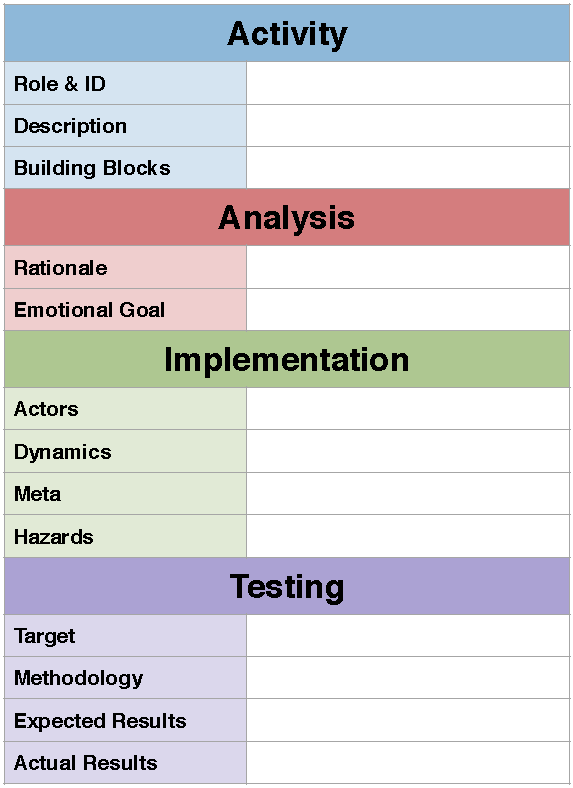
\includegraphics[width=6cm]{gamification/frame2}
\caption{Gamification Activity Template}
\label{fig-frame}
\end{figure}

Our framework is based on the concept of {\em Activity} (depicted in \figref{fig-frame}), which is composed of {\em Analysis}, {\em Implementation}, and {\em Testing}.
Each activity pertains to a specific user type (role), present in gamification systems, which can be \begin{inparaenum}[i)] {\em \item Observer}, who acts in read-only mode and does not contribute anything new, {\em \item Writer}, who only interacts by modifying existing contents and {\em \item Solver}, who accomplishes the objectives of the gamification system\end{inparaenum}.
People interacting with a gamification system dynamically switch between these roles.

An \textbf{Activity} consists of an {\em ID} formed by the initial letter of the role plus an incremental number (\eg the first activity listed in Writer has the ID ``W1''), a brief {\em description}, and a list of pertinent gamification building blocks (which we describe later).
Each activity is structured in the following way:

\begin{enumerate}

\item{\textbf{Analysis:}} Each activity within the gamification environment must come with an easily understandable {\em rationale} to connect to the global objectives of the environment, and the {\em emotional goal} we want to achieve in the people.
Without this analysis step, a gamification effort risks turning into a random set of arbitrary decisions.

\item{\textbf{Implementation:}} To implement an activity the {\em actors} must be known and we need to understand which gamification {\em dynamics} they will be involved in, which represent the tactics to engage people in a specific activity.
This is instantiated with game components we call {\em meta}, following Taje's nomenclature.
Last, one must ponder the {\em hazards} that can arise from a game structure (algorithmic issues, misbehavior, hardware requirements, \etc).

\item{\textbf{Testing:}} The last component is devoted to testing the activities, where it must be understood which entities are the {\em target} of the testing, which {\em methodology} can be used to perform the testing, and lastly, which the {\em expected results} and the {actual results}, to facilitate an iterative approach to the development of a gamification environment.

\end{enumerate}

This description of the framework is given from a conceptual point of view, obtained through several iterations and pilot tests we do not describe due to space constraints.
Before we can provide concrete examples of how the framework is to be used, we need one last missing and fundamental piece: Each activity hinges on one or more {\bf building blocks}, which also denote the particular categories of gamification it belongs to.

%%%%%%%%%%%%%%%%%%%%%%%%%%%%%%%%%%%%%%%%%
\subsection{Gamification Building Blocks}\label{sec:gamification-building-blocks}

The ten building blocks we present here have been identified during the construction of several software engineering gamification environments we have constructed, and which we briefly present in a latter section.
We do not claim the list of building blocks is exhaustive, but after constructing the aforementioned gamification environments we did not see other building blocks emerge from our efforts.
The building blocks are denoted by a series of aspects recurrent in the literature: According to Werbach and Hunter players {\em go through a journey}, progressing through an environment, first by ``on-boarding'', then by ``scaffolding'', and later by achieving ``mastery''~\cite{Werb2012a}.
Adopting Lazzaro's ``keys to emotions''~\cite{Lazzaro2004}, good emotions triggered by solving puzzles, accepting challenges, and designing strategies are elicited by {\em hard fun}.
Moreover, the {\em people factor}, which stems from socializing and working with people and giving/receiving gratitude is fundamental in community-based gamification environments.
Embracing Seligman's concept of {\em resource building}~\cite{seligman2000positive}, it is beneficial to provide some form of avatar of the player which matures and grows as the gamification environment is being explored.
This in turn is tied to the concept of ``leveling up'' described by McGonigal~\cite{McGo2011a}.

Before coming to the ten building blocks, one further consideration: As opposed to existing gamification environments, one which is tailored for software engineering must include the possibility of dynamically adapting itself.
Since software systems are developed for very long periods of time, even decades, an environment should feature the possibility of removing existing rewards and adding new ones as the environment is being used.

\buildingblock{Portal}{portal} When users cross the boundaries of the gamified platform, they register a profile and provide information that describes them to the virtual community.
Despite being a trivial operation, it has a relevant feature: It is the very first action that users accomplish in entering the new world, and should be acknowledged with a reward.
{\em Example:} Bob registers to the Bug Tracker and receives a ``Welcome'' badge.

\buildingblock{Production}{production} After registering, users must become immediately productive in the environment, because delays in starting using the platform may result in a drop of interest and cause users to quit.
We split this block into three sub-blocks, according to the ways in which users have the possibility to produce content and receive rewards.
\begin{itemize}
  \item \textbf{Symbiosis}: performing an activity that directly or indirectly helps someone else's activity or state.
Acting well in favour of others benefits both parties.
{\em Example:} Bob provides useful comments to a bug being handled by someone else.
  \item \textbf{Narcissus\footnote{Narcissus was a Beotian hunter in Greek mythology who was so proud of his feats that he fell in love with his own image reflected in a pool.}}: doing something to self-improve one's position in the community.
This action helps users to understand the structure and  mechanisms of the community.
{\em Example:} Bob provides his first bug fix.
  \item \textbf{Hive}: proposing an idea to improve the platform and community life.
{\em Example:} Bob proposes to introduce a ``Bug of the day'' notification mechanism.
\end{itemize}

\buildingblock{Bravery}{bravery} In the production process, users may attempt hard tasks.
The more skilled they become, the more confidently they will attempt to achieve bigger goals.
Such bravery leads to important achievements and should be equally rewarded.
{\em Example:} Bob fixes an old bug that made many people despair and is awarded by the community with an ``Unstoppable'' badge.

\buildingblock{Scrum}{scrum} In Rugby, Scrum is a way of restarting the game: Players bind together in order to make the other team collapse and take possession of the ball.
The key is to rely on the strengths of everyone.
Cooperating, collaborating, sharing useful tools, competing against, socializing with other community members is intrinsically motivating.
The system should reward and promote teamwork.
{\em Example:} Bob spends time assigning bug reports to users that he knows to be expert in the area, or tagging easy bugs for newbies.

\buildingblock{Chameleon}{chameleon} While gaining skills and experience, the user may do something unique, spectacular, or never tried before.
The environment should react by introducing a new achievement and release an ad-hoc reward, which becomes part of the gamification library of the system and achievable by other users.
Conversely, if a specific reward has never been reached by any user for a long time, the reason might be its impracticability; the system should dynamically remove such an achievement from the library.
We affiliate such a dynamism with the ability of chameleons to change their own skin colour according to the surrounding environment.
{\em Example:} Bob closes five bug reports with a single fix.
The system administrators create a special ``Epic'' badge, and add it to the possible badges users can achieve.

\buildingblock{Thunderbolt}{thunderbolt} When users become experts, with many obtained rewards, they might fall into a state of boredom.
The result is decreased motivation and productivity.
To awake them from inactivity, the system should hit them like a thunderbolt with an announcement and direct them toward a new challenge, such as a one-week long quest where contestants can be awarded custom prizes.
This should spur many users to participate.
{\em Example:} Bob has not participated in any bug fixing activity for the last month.
He and similar users are notified about a complex bug and a bounty for fixing that bug.

\buildingblock{Phasing}{phasing} Users may perform actions in the virtual world that, in reality, produce a permanent impact on the surrounding.
Phasing suggests to mutate the environment according to the progression of each user's expertise.
Two users, at different stages of their progression  see different representative phases of the same scenario and can interact with it in different ways.
{\em Example:} Bob tags bugs that are old and inactive, but still interesting.
The administrator then creates a new section highlighting such bugs, and acknowledges the contribution of Bob.

\buildingblock{Beautification}{beautification} Appearance, even if only virtual, is important to many.
The users' avatars change appearance over time and become more appealing as they progress in the environment.
In the opposite case of inactivity, the appearance of the avatars starts to slowly degrade.
{\em Example:} As Bob becomes an expert bug fixer, his avatar (for example depicted as a warrior) is decorated with better clothes and weapons.
After a period of inactivity due to his (real) holidays, Bob's avatar is depicted out of shape and with a broken sword.

\buildingblock{Champagne}{champagne} Since achievements inside the magic world are important to users, they want to celebrate their success not only within the virtual world, but also in the real one.
{\em Example:} Bob is looking for a new job and on his curriculum puts a link to his profile in the bug tracker, as proof of his expertise\footnote{Mozilla is already proposing a similar concept at http://openbadges.org/}.

\buildingblock{Ascension}{holyascension} A game usually has an end.
It is intrinsically rewarding and fulfilling to see the words {\em The end} on a screen, even though the actual satisfaction comes by what was done along the way.
This building block does not come with a reward, as otherwise inactivity might set in.
If users collected vast amount of rewards and participated in the community, they should be rewarded in the real world as well.
{\em Example:} Bob has been a productive bug hunter for many years, and is rewarded by the environment admins by being invited to become also an admin.\\

{\bf Putting everything together.} In the following we provide two concrete examples of gamification environments we have been developing.

%%%%%%%%%%%%%%%%%%%%%%%%%%%%%%%%%%%%%%%%%
\subsection{Example I: The Myth and De-Bug}\label{sec:gamification-example-bugs}

The objective is to develop a gamification system for a bug tracking system.
Fixing a bug is like struggling against a monster that threatens a village.
This image inspired the overall theme of ancient Greece, full of heroes, gods, legends, and epic battles with mythological beasts.
We set the following goals for a gamification system in bug reporting:
\begin{enumerate}[(1)]
	\item {\em improve the quality of bug reports:} we want to stimulate users to include meaningful information.
Zimmermann \etal showed that some elements are crucial to ease the fixing process, such as stack traces~\cite{Zimm2010a}.
	\item {\em stimulate the participation of the community:} we want to create a friendly environment for newbies and with engaging activities for experts.
	\item {\em ease the fixing process:} we want to reduce the time spent dealing with cumbersome information, to allow developers to spend their time in fixing the defects.
We want encourage users to deal with unsorted data in the tracker, like assigning bug reports to the appropriate user, closing duplicate reports, or highlighting important bugs.
\end{enumerate}

\textit{The Myth and De-bug} reflects the journey of a player that begins with the on-boarding phase, continues with some scaffolding, and terminates with mastery.
We produced a large set of activities, such as the one in \figref{fig-act2}.

%\begin{figure}[t]
%\centering
%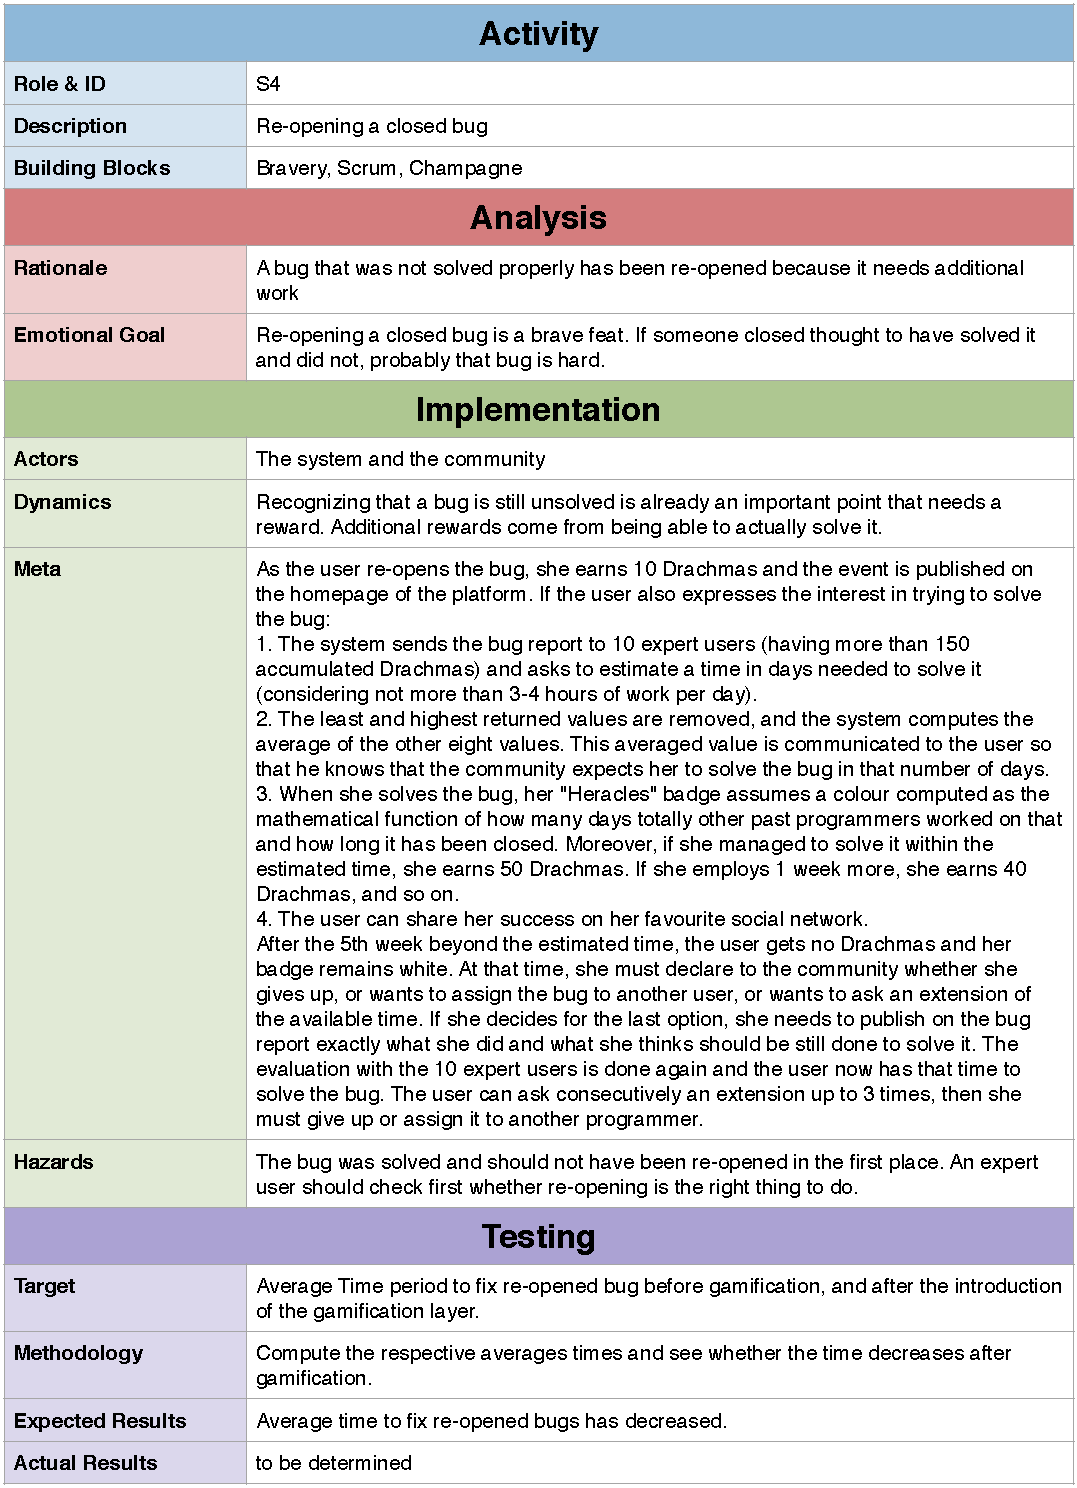
\includegraphics[width=7.7cm]{gamification/act2}
%\caption{Concrete Gamification Activity}
%\label{fig-act2}
%\end{figure}

Due to space reasons we cannot depict all activities; the goal is to clarify that creating activities is a lengthy process which must be done in an iterative way.

\badge{yob_badge} As the player signs up for the game, she enters the magic world of ancient Greece and receives her first reward, the \textbf{Newbie badge} and a small amount of drachmas (the ancient Greek currency), with which the player can buy her avatar some equipment.
The game awards different amounts of Drachmas according to the difficulty of the accomplished task.
This first operation is trivially easy (just registering and give some personal information for the user profile), but it has a special feature: It is the first action that the user does to get into the platform and the first active contact with the community.
Moreover, receiving immediately an unexpected reward works as a bait for the new player who is motivated to add another prize to her collection as soon as possible.

\begin{figure}[t]
\centering
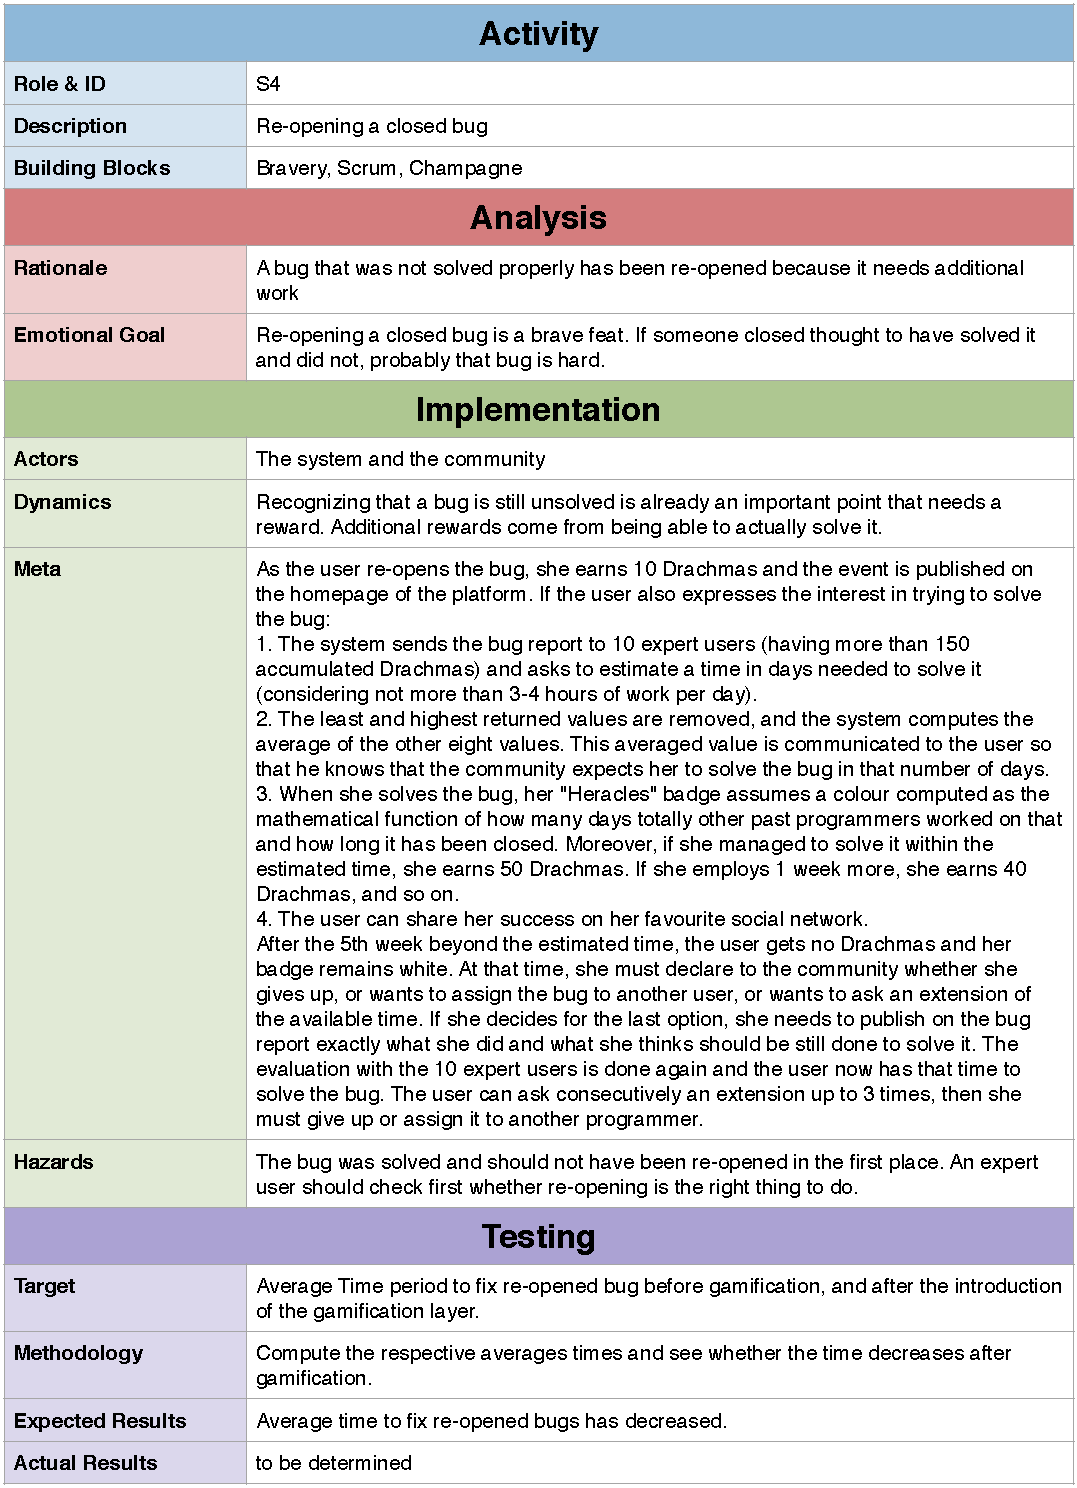
\includegraphics[width=.65\linewidth]{gamification/act2}
\caption{Concrete Gamification Activity}
\label{fig-act2}
\end{figure}

\badge{briefed_badge} The second unexpected reward is quite easy to acquire too: Becoming conscious of the rules holding in the world of Ancient Greece, the player earns the \textbf{Briefed badge}.
She does so by going through a tutorial which explains the bug tracker and the rules of the game.

The system assists the player along the whole path to mastery: It directly furnishes to the user practical tasks that she can afford with her current skills.
While writing a bug report, the system supports the player by using mandatory \textbf{box fields} asking for specific information or suggesting where to look to find it.
It helps reporters to not forget essential information and provides some scaffolding to boost player to mastery.
Motivation is a precious good that some techniques are able to elicit, but at the same time can be shut down easily.
A single apparently insignificant demonstration of disapproval from some other member of the community can hurt a newbie.
\textit{The Myth and De-Bug} avoids such an effect by impeding questions and answers with scores smaller than 0 and avoiding the so-called ``Dislike'' system.

\badge{phidias_badge} A point of strength of this gamification layer is that everyone, from the new user up to administrator, has the chance to propose improvements for the  environment.
The player whose proposal for an extension of the environment has been accepted by the community, gains the \textbf{Phidias badge}.

\badge{tombraider_badge} An open problem of gamification communities (for example Stack Overflow), is keeping the motivation of users high or to recover it when it naturally decreases~\cite{Grant2013}.
We designed badges that level up proportionally with the amount of work performed, \eg \textbf{Tomb Raider} is a badge achievable when a developer explores old posted reports, finds something interesting, and sets the status of the report back to active.

%\badge{heracles_badge}
\noindent
\begin{wrapfigure}{l}{0.07\textwidth}
  % \vspace{-2.5em}
  \vspace{-18pt}
  \begin{center}
    
\includegraphics[width=0.06\textwidth]{gamification/heracles_badge.pdf}
  \end{center}
  \vspace{-30pt}
\end{wrapfigure}
\textbf{Heracles}\footnote{Heracles was the greatest hero in Greek mythology.
He had incredible courage, physical strength and ingenuity.
Among the many ventures attributed to him, he defeated the Hydra monster, a sea serpent with nine heads.
Every time someone cut one away, it grew anew.
This is a conceptual parallelism with what happens with closed bugs that are reopened.} is a badge of the same nature of Tomb Raider, but is awarded for closing re-opened bugs.

% \pagebreak
Our environment also deals with the issue of {\em balance}.
If a gamification layer is too linear in terms of dispensing mere (and in a way meaningless) points, the danger of pointsification comes up: Users start to hunt for points by performing meaningless and contradictory actions, such as re-opening bugs that do not need to be reopened.
The building block {\em Scrum} is crucial in this case, which means to rely on the community, for example by setting time limits for specific activities.

Also, our environment does not make large use of leaderboards because they are gamification elements that, in a number of cases, may demotivate players.
We designed the leaderboard ``Twenty Top Hoplites of The Week'' by relying on the fact that having a considerably high work rate is an occasional ability.
Since a developer cannot be constantly productive, the leaderboard thus becomes dynamic.

\badge{achilles_badge} When users are on the leaderboards for an extended period of time, they gain the \textbf{Achilles\footnote{We choose for this badge the figure of Achilles, the king of the Myrmidons, son of Zeus and Thesis.
The parallelism with the badge comes from the fact that his most common epithet in Homeric works is ``swift-footed'' because Achilles was known to be very fast at running.} badge} and an amount of bonus Drachmas to refurbish the avatar.

To foster epicness, one of the traits identified by McGonigal as instrumental to gamification, our environment provides a number of places where players can acknowledge the feats of other players.
This happens for instance when a developer closes a difficult bug, or the community reaches a landmark (\eg closing the 1000th bug) collaborating as a team.
The environment also features specific leaderboards, in the form of halls of fame, where important contributors are acknowledged or where productive former newbies are entered into the category ``The New Greek Legends''.

\textit{The Myth and De-bug} is an instance of inducement prizes: Its goals are efficiency, development of creativity, and stimulating collaboration among the community even while competing.
It is also ``cheap'' because it only involves virtual goods, and pays a deep attention to balancing issues.
We just described a possible instantiation of this gamification system.
We could take exactly the same framework, substitute the name of the badges and imprint the game toward modern heroes (Spider Man, Batman, Superman, etc).
They are just fancy names, and we can use the fantasy we like to shape the same gamification dynamics.

\subsection{Example II: The Empire of Gemstones}\label{sec:gamification-example-gems}

The first example was developed in the context of a novel bug tracker we are implementing~\cite{DalS2014a}.
We also devised a number of other software engineering gamification environments, which led to the distillation of the building blocks discussed previously.
We now present another case study of a gamification layer for a software engineering context: Modern Code Reviews.
Due to space limitations we do not present the solution at the same level of detail as the previous example, but focus here mostly on a concept that was only sketched in the previous section: \emph{leveling up}.

Code reviews is a software engineering practice that consists in manually reviewing source code written by other people, to verify and improve the quality of the code.
While the effectiveness of this method has been proven during the years~\cite{Shull2008a}, this practice is often considered expensive, cumbersome, and, as such, difficult to adopt.
Bacchelli and Bird proposed \textit{Modern Code Reviews}~\cite{Bacc2013a}, a code review approach that is informal, tool based, and performed on a frequent basis.
They developed \textit{CodeFlow}, a tool where the user can annotate the source code and interact with other users with a chat.
A developer that wants to propose his code for review has to create a package with the changes, write a brief description and submit it to the \textit{CodeFlow} service.

The area of code reviews still has many open questions, but the \textit{CodeFlow} platform represents the ideal environment to develop a gamification layer to stimulate the amount of motivation necessary to turn code reviews into a habit.

In the context of a code review tool we are currently building in the research group, we designed a gamification environment named \textit{The Empire of Gemstones}, to exploit the parallelism between collecting gemstones and improving the quality of the code.
We employ gems as a virtual currency to reward positive feedback while using proposed solutions.
The number and the type of gems compose a reputation system based on noble titles, used by the system to rank users, which also facilitates the finding of experts in specific areas.

It has been shown~\cite{Bacc2013a} that teams use code reviews for the following purposes: (1) finding defects in the code; (2) improving the code; (3) finding better implementations; (4) transferring knowledge in the group; (5) increasing the team awareness and transparency; and (6) sharing code ownership.

Given the strong implicit collaborative nature of code review tools, we pose a strong accent on blocks that expect interaction with other users, like \emph{Scrum} and \emph{Champagne}.
However, also the motivation of single users can be catalyzed, for example by rewarding quality code, thus suggesting the use of \emph{Bravery} and \emph{Thunderbolt} blocks.

In parallel with a set of badges devised with a similar procedure to the one used to build \textit{The Myth and De-Bug}, we introduce a ``leveling'' mechanism to provide users with a feeling of progression and growth while reviewing the code: Leveling is one of the main drivers of gamification systems, as it fosters positive competition among the players.

By reviewing other's code, a user gets a gem.
The kind of gem depends on the number, size and difficulty of the reviews.
Each gem has a different value according to its rarity, as we see in \tabref{tab-gems}.

\begin{table}[ht]
\begin{center}
\caption{Points acquired per 1 gemstone.}
\begin{tabular}{l|r}
\textbf{Gemstone} & \textbf{Points} \\
\hline
\rowcolor{emerald}Emerald & 10\\
\rowcolor{sapphire!40}Sapphire & 9\\
\rowcolor{tanzanite}Tanzanite & 8\\
\rowcolor{aquamarine}Aquamarine & 7\\
\rowcolor{ruby}Ruby & 6\\
\rowcolor{jade}Jade & 5\\
\rowcolor{citrine}Citrine & 4\\
\rowcolor{topaz}Topaz & 3\\
\rowcolor{amethyst}Amethyst & 2\\
\rowcolor{quartz}Quartz & 1\\
\hline
\end{tabular}
\label{pointsgem}
\label{tab-gems}
\end{center}
\end{table}

For example, a reviewer may check some code that includes changes for fifty lines of code over five different files, for which she receives a Jade.
Another user reviews three small changes, each one involving only one file, and she receives three Quartz.
Reviews that spot bugs, that propose a better implementation of the reviewed code (goals 1, 2 and 3) get higher value gems, but since reviewing code also means knowledge transfer (goal 4 and 5), users get a reward even if the review causes no changes.

Submitting code for review implies willingness to collaborate and accept critics, an not being protective of her code (goal 6).
We decided however not to assign gems depending on the outcome of the review to the submitter, to avoid pointsification and because that would suggest an idea of code reviews begin judgmental, which in the long run would discourage a user from submitting his code for review.
A submitter can however still receive badges for particular behaviors, like the \textbf{Collector} badge for users that submit regularly their code, or the \textbf{Houskeeper} for users that submit large numbers of reviews in a short time.

By collecting gems, a user can grow his estate and obtain noble titles which reflect the expertise level in the community, as depicted in \tabref{tab-noble}.
For example, a new user in the team is reviewing many small changes to understand the project he is working on.
He then collects many Quartz, slowly being promoted to Knight after 12 reviews, and Baron after 24.

\begin{table}[t]
\begin{center}
\caption{Required number and type of gemstones to obtain noble title.}\label{titles}
% \begin{tabular}{p{0.5cm}p{0.7cm}p{0.7cm}p{0.7cm}p{0.7cm}p{0.7cm}p{0.7cm}p{0.7cm}}
\begin{tabular}{rrrrrrrr}
& \multicolumn{7}{c}{\textbf{Noble Titles}}\\
\cline{2-8}
\multicolumn{1}{l|}{\textbf{Family}} & \cellcolor{gold!100} Prince & \cellcolor{gold!84} Duke & \cellcolor{gold!74} Marquis & \cellcolor{gold!64} Count & \cellcolor{gold!52} Viscount & \cellcolor{gold!40} Baron & \cellcolor{gold!28} Knight\\
\hline
\rowcolor{emerald} \multicolumn{1}{l|}{Emerald} & 27 & 21 & 16 & 12 & 9 & 6 & 3\\
\rowcolor{sapphire!40} \multicolumn{1}{l|}{Sapphire} & 34 & 27 & 21 & 16 & 12 & 8 & 4\\
\rowcolor{tanzanite} \multicolumn{1}{l|}{Tanzanite} & 41 & 33 & 26 & 20 & 15 & 10 & 5\\
\rowcolor{aquamarine} \multicolumn{1}{l|}{Aquamarine} & 48 & 39 & 31 & 24 & 18 & 12 & 6\\
\rowcolor{ruby} \multicolumn{1}{l|}{Ruby} & 55 & 45 & 36 & 28 & 21 & 14 & 7\\
\rowcolor{jade} \multicolumn{1}{l|}{Jade} & 62 & 51 & 41 & 32 & 24 & 16 & 8\\
\rowcolor{citrine} \multicolumn{1}{l|}{Citrine} & 69 & 57 & 46 & 36 & 27 & 18 & 9\\
\rowcolor{topaz} \multicolumn{1}{l|}{Topaz} & 76 & 63 & 51 & 40 & 30 & 20 & 10\\
\rowcolor{amethyst} \multicolumn{1}{l|}{Amethyst} & 83 & 69 & 56 & 44 & 33 & 22 & 11\\
\rowcolor{quartz} \multicolumn{1}{l|}{Quartz} & 90 & 75 & 61 & 48 & 36 & 24 & 12\\
\hline
\end{tabular}
\label{tab-noble}
\end{center}
\end{table}

The avatar of the player in this environment is then also depicted in a gameful way, such as a house which gets more beautiful as the player obtains more gems.
In the code review tool, these avatars could then be shown to other reviewers when they log into the tool.

As we anticipated, the leveling mechanism is useful in stimulating positive competition among team members.
Given the context of code reviews, which by definition happen inside the same team, company or community, we believe that the level system is particularly effective in leveraging the interpersonal bonds and endorse motivation in improving the quality of the code.


%%%%%%%%%%%%%%%%%%%%%%%%%%%%%%%%%%%%%
\section{Evaluating Gamified Systems}\label{sec:gamification-evaluation}
%%%%%%%%%%%%%%%%%%%%%%%%%%%%%%%%%%%%%

Once a system is gamified, we need to be able to measure the impact of the gamification, and how much it contributed to reach the {\em business objectives}.
It is crucial not to confuse business objectives with game objectives: with the coexistence of ``serious'' and ``fun'' layers, it is easy to exchange the goals of the two aspects, thus misjudging the effects.

In building our framework, we included a testing section, whose purpose is to decide at design time a procedure to state how successful the game elements applied to each single activity are.
But, a system is more than the mere sum of all its parts: As such, testing all the single elements does not imply the success of the whole gamification system, exactly as in software development we need integration tests.

We propose five methods to assess the general performance of the gamification on top of a software engineering context: \emph{success metrics}, \emph{analytics}, \emph{conflicts}, \emph{jen ratio} and \emph{survey}.
The first three focus on technical aspects to consider the business objectives, while the the last two consider emotional aspects.
Due to their subjective nature, we cannot get a precise measure of emotional response of the users and compare the obtained values in a consistent way.
The relative metrics have then to consider the imprecise nature of the data they deal with.


\subsubsection{Success Metrics}

The first approach is to define a set of goals at design time, and verify them after the system has been in production for a while.
We recommend to make a list of the goals of the gamification system, define success metrics (number of new users in the last month, average activity increase per user, \etc) tailored to specific activities and verifiable with usage data.
A long enough timeframe must be used to perceive a noticeable change: People's habits take a while to deal with novelties.
A significative amount of data must be collected before and after the introduction of the gamification layer to enable before/after testing.


\subsubsection{Analytics}

A useful metric is represented by the measure of users interacting with the enviroment: \emph{Daily Active Users (DAU)} is the number of unique users that interact with the software tool during a day, while \emph{Monthly Active Users (MAU)} is the average number of unique users that interacted with the software tool in the previous 30 days.
By computing the ratio $\frac{\textit{DAU}}{\textit{MAU}}$ we have the trend of usage of the software tool in a given moment.
The result of such a ratio goes from 0 to 1: It is close to 1 when the tool is engaging, and it is close to 0 when its popularity is decreasing.
$\frac{\textit{DAU}}{\textit{MAU}}$ is a relevant parameter to keep under observation because, if it increases the number of active users is growing; if it decreases they are decreasing.


\subsubsection{Conflicts}

Some gamification elements can create conflicts with existing elements on the system.
Listing and prioritizing the conflicts, also by listening to the users through forums and mailing list, is helpful.
If a conflict persists, the involved gamification elements should be pulled out of the environment, as user dissatisfaction can be harmful to the whole community.


\subsubsection{Jen Ratio}

Establish two sets of interactions in the user community: \emph{positive interactions} (\eg virtual gifts, acknowledgements), and \emph{negative interactions} (\eg misbehaviours, rude comments).
Compute the \emph{Jen Ratio}: total positive interactions among users over the total negative interactions, in a given period of time and context.
The outcome is between 0 and 1.
The jen ratio assesses how positive the attitude of the users is: the closer to 1, the better the social well-being of the community.


\subsubsection{Survey}

Selected users, of all expertise levels, should be periodically surveyed, where key questions should not only regard technical aspects, but also emotional aspects.


\subsubsection{}

Beyond the use of these metrics, it is important to perform an evaluation on the effective gain of the system, to quantify how the use of gamification impacted the activity of the users and if it brought actual benefits.
For example, in a bug tracking system we can measure the number of bug reports opened and closed every day, the average duration of a bug report and the number of bug reports that a user examines.
However, it is clear that such metrics are domain specific, and have to be calibrated for each different gamification context.


%%%%%%%%%%%%%%%%%%%%%%%%%%%%%%%%%%%%%%%%%%
\section{Summary}\label{sec:gamification-summary}
%%%%%%%%%%%%%%%%%%%%%%%%%%%%%%%%%%%%%%%%%%

We presented a critical overview on the relevant literature on gamification, and proposed a framework to support the design of a gamification layer to support software engineering tasks.
We showed how to implement practical actions to successfully gamify a system, and we distilled ten essential \emph{building blocks} that represent basic elements to be considered when designing gamification activities.
We then discussed two example software gamification environments we are currently building, highlighting a number of challenges.
Last, we outlined a proposal on how gamification systems can be evaluated.

\subsection{Reflections}

The examples in \secref{sec:gamification-framework} hint at a fact that should not be disregarded about gamification: To create such environments is a far from trivial endeavour.
The reasoning that goes into creating thematic environments, the way that leveling is handled, how and when awards and badges should be assigned, is a strongly iterative process.
One might be tempted to bypass such a labor-intensive work by using the simplest solution, which is to award points and to base the leveling on such points.
However, apart from the danger of pointsification, there is another risk, which we define as ``stalling'': If the gamification layer is not constantly revisited, maintained, and evolved, it risks to quickly become obsolete, and therefore will not only be ignored by the users, but it might even cause decreased participation.
Last, there is also the issue of adoption: Since many software engineering activities are done with tools that come from vendors or open-source communities, one would have to convince those to introduce the gamification layer on top of their tools.
It is doubtful that this would happen if there is no substantial evidence that the gamification layer actually works, which brings us back to the concern of evaluating such environments.

% \subsection{Related Work}
%
% There have been few other efforts in this direction so far.
% Passos \textit{et al.}~\cite{PassosMNC11} proposed to gamify the phases of software lifecycle by splitting the whole process into tasks, and setting achievements for their completion.
% While this is an interesting approach, it is essentially a \emph{pointsification}, and as such puts too much emphasis on the rewards, thus being ineffective on the long run.
% Singer and Schneider performed a study on the gamification of commit messages~\cite{sing2012}: they managed to influence the workflow of the students in the experiment, improving the workflow.
% They however received both positive and negative comments.
% Dubois and Tamburelli~\cite{Dubois2013a} pointed out that software projects often produce mediocre quality artefacts, do not respect the terms for milestones, or exceed the financial budget.
% They claimed that gamification could represent a solution to the issue, but only outlined a possible approach to gamification based on the three steps analysis, integration, and evaluation.
% Probably still being in the inception phase they did not provide concrete suggestions or a systematic set of recommendations.
%
% We believe this paper provides a starting point to approach the gamification of software engineering in a systematic way and also provided recommendations on how to evaluate it.

\subsection{Next Steps}

We composed the gamification layers presented in this chapter as part of the process to understand the basic concepts of gamification and practically see what is meaningful or what should be highlighted as dangerous.
The main result of our work were the gamification framework and the ten essential building blocks to use as a reference in building the system, but the presented scenarios are actual software engineering problems currently investigated by researchers.

The focus of our work revolves around the activities performed by the users.
However, further insight can come from considering the different types of users in a community, to avoid the negative effect of marginalizing some users.
For example, Vasilescu \etal studied the difference between men and women in approaching---and leaving---a community~\cite{vasi2012}, while Koivisto \etal showed how the ease of use of gamification tends to decline with age~\cite{koiv2014}.


%The solutions developed to build \textit{The Myth and De-Bug} were designed with an actual use scenario in mind, and are being integrated into \textit{ShoreLine}, a comprehensive platform to manage bug reports developed for the \textit{Pharo}\footnote{https://pharo.org} community.
%\textit{Pharo} is a programming language inspired by \textit{Smalltalk}, with an active development and an energetic community.
Our hope is that integrating gamification elements in software engineering will allow developers to build tools where the potential of gamification is leveraged to foster collaboration and contributions by the community.
In that sense: The game has just started.
